\documentclass[class=book, crop=false, oneside]{standalone}
\usepackage[subpreambles=true]{standalone}

\usepackage{../../style}
\usepackage{../../set-citations}

\graphicspath{{./assets/images/}}

% arara: pdflatex: { synctex: yes, shell: yes }
% arara: latexmk: { clean: partial }
%! arara: clean: { extensions: [sta] }
\begin{document}
\chapter{I/O}\begin{fquote}[Elayne Boosler]I am thankful the most important key in history was invented. It's not the key to your house, your car, your boat, your safety deposit box, your bike lock or your private community. It's the key to order, sanity, and peace of mind. The key is "Delete".
 \end{fquote}

\section{La necessità di comunicare}
Un calcolatore sarebbe praticamente inutile se non avesse la possibilità di interfacciarsi e comunicare con l'esterno, ed è proprio di questo che si occupano le periferiche di input/output (da qui in avanti I/O); questi dispositivi possono essere estremamente \emph{eterogenei} tra loro e si diversificano a seconda del compito che sono chiamati a svolgere\footnote{Si pensi che nella categoria di dispositivi I/O compaiono mouse, penne grafiche, desktop, microfoni e tanti altri ancora.}. Tuttavia devono avere una caratteristica comune: devono essere \emph{espandibili}, ovvero ci deve essere la possibilità di aggiungere o rimuovere i dispositivi di I/O.

\subsection*{Tre termini tecnici}
Chiariamo ora questi termini tecnici definendone precisamente il significato poiché ci torneranno utili nel resto del capitolo.
\begin{itemize}
	\item \emph{Transizione di I/O}: invio indirizzo e spedizione o ricezione dei dati.
	\item \emph{Input}: trasferimento di dati da una periferica verso la memoria dove il processore può leggerla.
	\item \emph{Output}: trasferimento di dati dalla memoria ad un dispositivo.
\end{itemize}
Data l'enorme varietà di compiti che assolvono le periferiche di I/O a  seconda del tipo di applicazione, posso essere interessato a diverse prestazioni:
\begin{itemize}
	\item in alcuni casi la cosa più importante è il tempo di accesso/risposta (latenza), ad esempio quando si tratta di tastiere o mouse;
	\item in altri casi la caratteristica di spicco deve essere il throughput, vedi i sistemi di streaming;
	\item infine esistono molti altri casi meno comuni che necessitano di caratteristiche dedicate (ad esempio un sistema bancario può avere la necessità di massimizzare il numero di file di piccole dimensioni su cui opera contemporaneamente).
\end{itemize}
Dati questi esempi si possono introdurre le principali caratteristiche secondo cui vengono suddivise le suddette periferiche: operazioni possibili (R e/o W), \emph{partner} (uomo o macchina) e velocità di trasferimento; in seguito viene riportata un tabella riassuntiva delle maggiori classi di dispositivi di questo tipo.

\begin{figure}[!h]
	\centering
	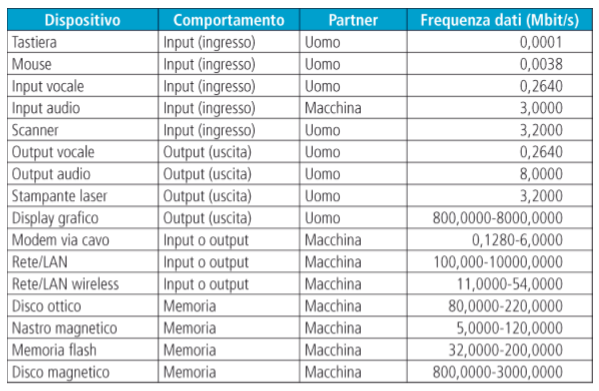
\includegraphics[width=0.9\textwidth,keepaspectratio]{classificazione-periferiche}
	\caption{Classificazione delle periferiche}
\end{figure}

\section{Connesione tra processore e periferiche}
Nonostante le differenze di cui si è parlato nella sezione precedente, tutte le periferiche hanno una caratteristica comune: la modalità di collegamento al processore. Vediamo ora uno schema, molto semplificato, che rappresenta il modo in cui le periferiche sono collegate al processore:
\begin{figure}[!h]
	\centering
	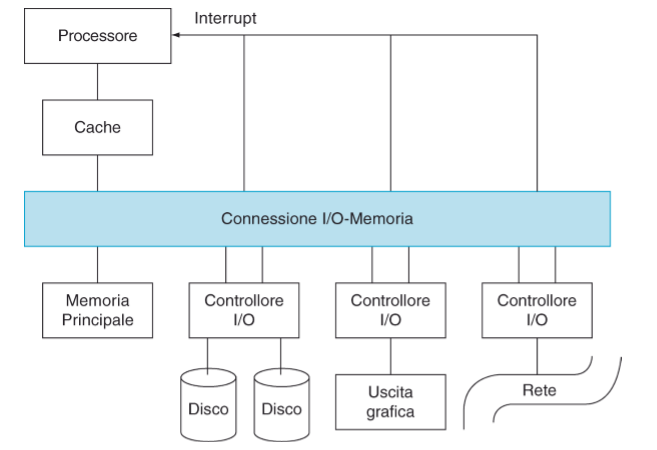
\includegraphics[width=0.9\textwidth,keepaspectratio]{schema-periferiche}
	\caption{Schema del collegamento delle periferiche}
\end{figure}
Si noti quindi come ogni periferica non è collegata direttamente con il processore, la loro comunicazione è intermediata dai controllori I/O e dal bus, che descriveremo in seguito.
Ciò implica che i dispositivi di I/O "non esistano" per il processore ma vengano rappresentati "virtualmente" come normali locazioni di memoria.

Tutte le connessioni avvengono attraverso strutture di comunicazione dette \emph{bus}. Ne esistono principalmente due tipologie:
\begin{itemize}
	\item \emph{bus processore/memoria}: sono specializzati, corti e molto veloci;
	\item \emph{bus I/O}: sono utilizzati per la comunicazione con periferiche generiche, possono essere relativamente lunghi e comunque non si interfacciano direttamente con la memoria, ma richiedono come intermediario un bus processore/memoria o un bus di sistema\footnote{Il bus di sistema è un "bus di alto livello", ovvero un bus dedicato a  mettere in comunicazione tutti gli altri bus del sistema appunto.}.
\end{itemize}
Nelle prime semplici architetture avevamo un unico grosso bus parallelo (non seriale) che collegava tutte le componenti, ma per problemi di clock e frequenze ora si usano architetture di comunicazione più complesse fatte di più bus paralleli condivisi e di bus seriali punto/punto\footnote{I bus seriali punto a punto sono bus in cui ogni periferica è collegata direttamente al processore tramite un bus dedicato.}.

Nel caso in cui il processore comunichi con delle periferiche esterne, come anticipato in precedenza, esso in realtà comunica attraverso i controllori I/O, che traducono sia i comandi che i dati da e verso il processore stesso.
Saranno ora discusse due implementazioni diverse del bus che convivono nei nostri calcolatori: \emph{sincrona} ed \emph{asincrona}.

\subsection{Bus sincrono}
Si tratta di un bus attraverso cui le informazioni vengono trasmesse in modo sincrono, quindi le comunicazioni sono necessariamente scandite da un segnale di bus clock (che gira a frequenza molto più bassa di quello del processore), che viene trasmesso in una linea di controllo del bus stesso.

\begin{figure}[H]
	\centering
	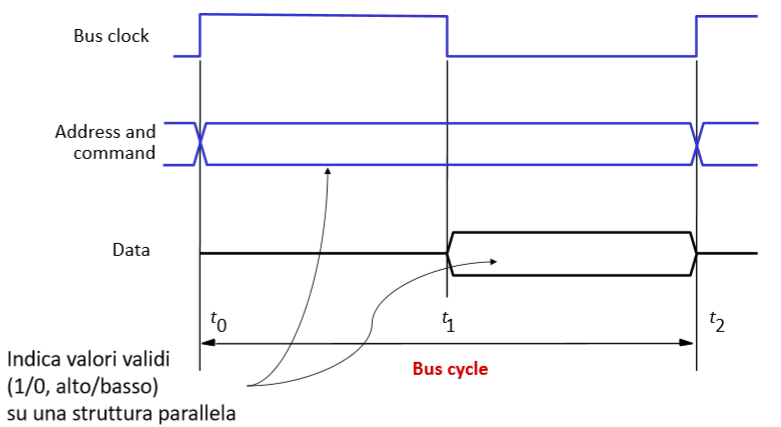
\includegraphics[width=0.9\textwidth,keepaspectratio]{bus-sincrono}
	\caption{Schema rappresentativo del ciclo del bus sincrono}
\end{figure}

In questo esempio si può osservare come avviene la trasmissione di un dato. Nell'\emph{Address and command}, durante il fronte di salita del bus clock, sono trasmessi indirizzo bersaglio e comando da svolgere, sul fronte di discesa del bus clock viene effettivamente trasferito il dato.
Il trasferimento termina proprio con il termine del ciclo di clock, in seguito il ciclo ricomincia; ripetendo ancora una volta per maggiore chiarezza, la prima metà del ciclo di bus clock è utilizzata per passare l'indirizzo e l'istruzione da svolgere, la seconda effettivamente per trasmettere il dato.

Riassumendo quindi i punti di forza del bus di tipo sincrono, si deve osservare che questo sistema è tanto semplice da implementare quanto veloce, data la presenza esigua di sequenze di controllo, che quindi non appesantisce lo svolgimento delle operazioni di trasmissione dati.

Di contro si può argomentare che è un sistema che dimostra poca robustezza al \emph{drift} del clock, ovvero se il dato non si propaga in modo sincrono con il  termine del bus clock e quindi viene trasmesso in modo scorretto; inoltre utilizzando un sistema simile si costringono tutte le periferiche a lavorare alla stessa velocità del clock, ma questo non è sempre possibile.

\subsection{Bus asincrono}
Per ovviare agli sconvenienti appena discussi è stata sviluppata anche una versione asincrona della tecnologia del bus che sostanzialmente non si appoggia più sul clock per il controllo delle transazioni ma utilizza un protocollo in cui le varie fasi sono determinate da \emph{handshake}\footnote{Gli handshake sono segnali che vengono utilizzati come segnali di controllo sulla ricezione o l'invio di dati.}.

Questo cambio di stratagemma libera dalla limitazione del tempo scandito dal clock ma comporta la creazione di apposite linee di controllo per segnalare inizio e fine delle transazioni;
nonostante questa complicazione il bus asincrono garantisce un grande vantaggio, ovvero permette di collegare periferiche a velocità diversa.

\begin{figure}[!h]
	\centering
	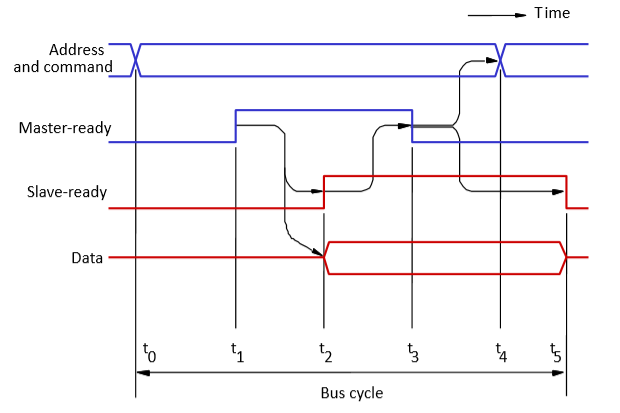
\includegraphics[width=0.9\textwidth,keepaspectratio]{bus-asincrono}
	\caption{Schema rappresentativo del ciclo del bus asincrono}
\end{figure}
Dall'esempio qui riportato si osserva che in ogni transizione una parte riveste il ruolo del \emph{master}, richiedendo delle operazioni, mentre l'altra parte fa da \emph{slave}, eseguendo i comandi.
Si nota quindi che esistono due linee di controllo dedicate (la master ready e la slave ready), che servono per trasmettere ai due componenti i segnali che indicano ad uno dei due che l'altro è pronto ed ha terminato la corretta trasmissione dei dati.

Riassumendo ora i punti di forza del bus asincrono, si noti che è un meccanismo che permette di avere un sistema robusto rispetto agli eventuali ritardi di una periferica rispetto ad un'altra o al processore e che consente di comunicare con periferiche di tipo diverso.

Viceversa, osservando i fattori negativi, si deve indicare che risulta più lento del bus sincrono data la necessità di inviare e ricevere diversi segnali di controllo ed inoltre, aumentando la complessità del trasferimento I/O, aumenta anche la complessità della circuiteria che sta alla base.

In conclusione, dando uno sguardo alla realtà, si scopre che spesso si usano tecnologie ibride di bus, in cui c'è un segnale di clock ma che rimangono prevalentemente asincrone.

\begin{figure}[!h]
	\centering
	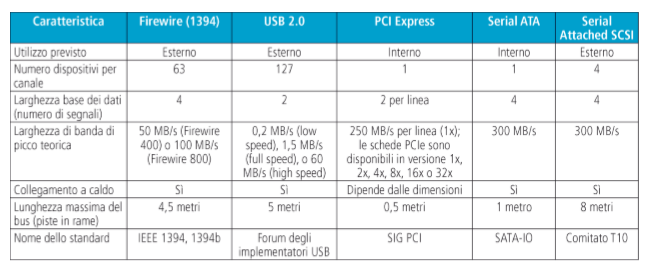
\includegraphics[width=0.9\textwidth,keepaspectratio]{tecnologie-asincrone}
	\caption{Principali tecnologie asincrone}
\end{figure}
Qui è ripotato un esempio di implementazione reale di questo schema. L'esempio riguarda l'ormai vetusta architettura dell'x86. Notiamo che esiste una componente dedicata alla comunicazione con tutte le periferiche, detto hub dell'I/O; Questo hub comunica poi in seguito con l'hub della memoria che si occupa di gestire le comunicazioni tra processore e memoria centrale oltre che interpretare le comunicazioni che arrivano apputno dall'hub dell'I/O.
Nei calcolatori moderni tutte queste componenti tendono ad essere inglobate nel processore stesso.
\begin{figure}[!h]
	\centering
	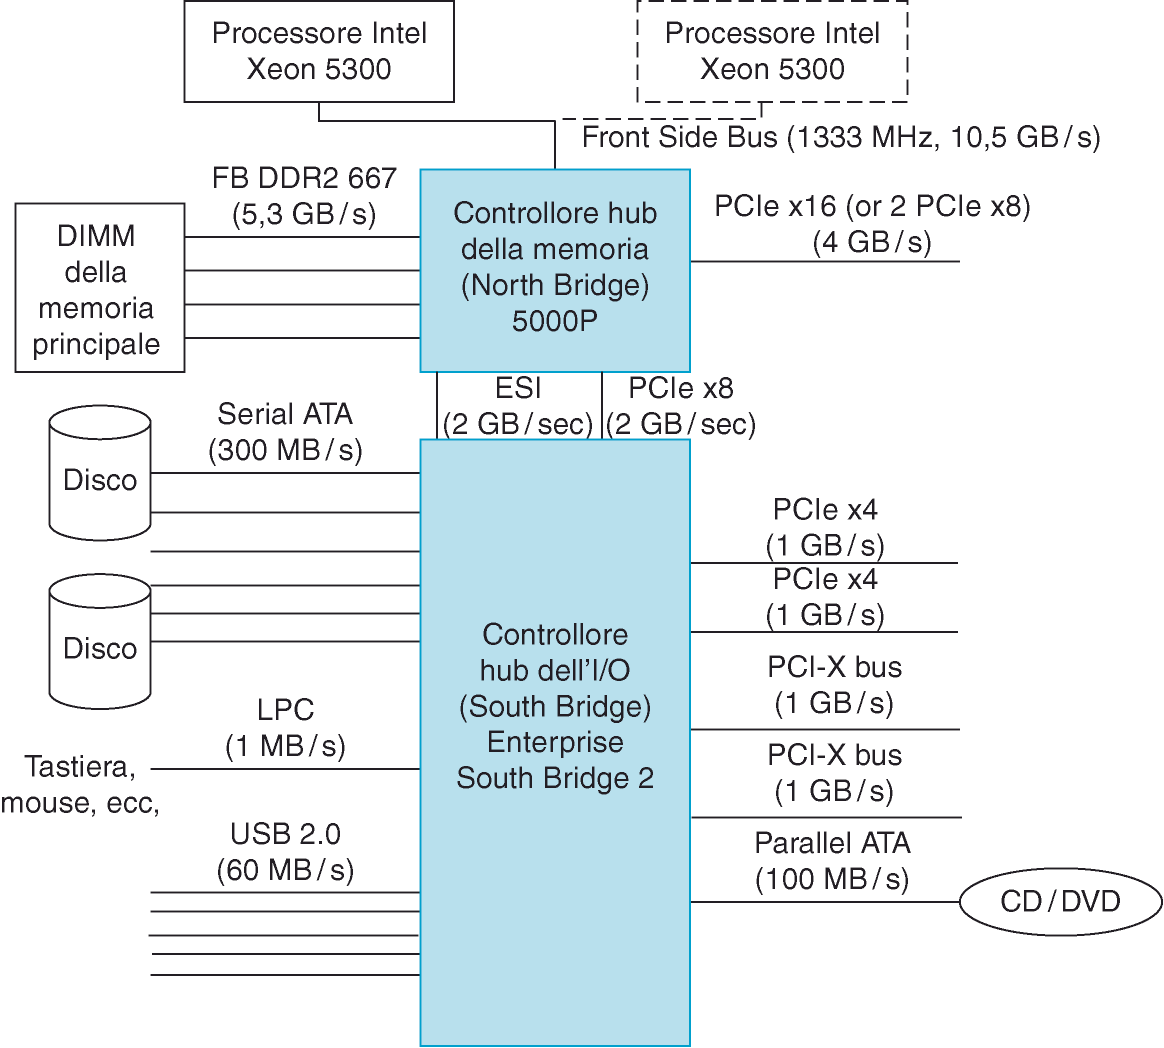
\includegraphics[width=0.9\textwidth,keepaspectratio]{esempio-x86}
	\caption{Schema collegamenti bus in x86}
\end{figure}

\section{Gestione delle periferiche da parte del SO}
Ora che abbiamo chiarito qual è il tramite fisico attraverso cui i sistemi operativi comunicano con le periferiche, rimangono ancora aperti i seguenti interrogativi: come trasformare una richiesta di I/O in un comando per la periferica? E come trasferire i dati? Di questi problemi si fa carico il sistema operativo (da qui in avanti SO), dato che è la parte di software dedicata alla gestione diretta del processore e delle sue risorse, quindi anche dei sistemi di I/O. Il SO deve fornire queste funzionalità per la gestione dell'I/O:
\begin{itemize}
	\item garantire che un dato utente abbia accesso ai dispositivi di I/O cui ha i permessi per accedere;
	\item fornire dei comandi di alto livello per gestire le operazioni di basso livello, trasferimento dati nello specifico;
	\item gestire le interruzioni generate dai dispositivi di I/O (in maniera simile a quanto avviene con le eccezioni generate nei programmi);
	\item ripartire l'accesso a ciascun dispositivo in maniera equa tra i vari programmi che lo richiedono.
\end{itemize}
È chiaro quindi, guardando il terzo punto, che i trasferimenti dati hanno un impatto sulle funzionalità del SO e di conseguenza vengono eseguite in una particolare modalità del processore, la modalità kernel.

Questa modalità è utilizzata per garantire la sicurezza delle operazioni assicurando, tra l'altro, che le comunicazioni siano atomiche (cioè che non avvenga più di un'operazione sulla stessa area di memoria nello stesso tempo).

Inoltre è evidente che per implementare le funzionalità appena elencate il SO deve poter inviare comandi alle periferiche, ricevere notifiche di corretta esecuzione dalle periferiche stesse e consentire trasferimenti diretti tra dispositivi e memoria. Nelle prossime sezioni sono discussi proprio i meccanismi che rendono tutto questo possibile.

\subsection{Come impartire comandi ai dispositivi}
Il sistema operativo impartisce comandi alle varie periferiche fornendo sulle relative linee di bus alcune "parole" di controllo attraverso due metodi possibili:
\begin{itemize}
	\item scrivendo/leggendo in particolari locazioni di memoria (memory mapped I/O);
	\item tramite alcune istruzioni speciali dedicate all’I/O.
\end{itemize}

Per chiarire questo meccanismo conviene procedere tramite un esempio:
memorizzando una particolare parola in una locazione di memoria associata al dispositivo il sistema di memoria ignora la scrittura, mentre il controllore di I/O intercetta l’indirizzo \emph{particolare} e trasmette il dato al dispositivo sotto forma di comando.

Queste particolari locazioni di memoria sono inaccessibili ai programmi utente ma solo il sistema operativo può operarvi, esso viene invocato tramite una chiamata di sistema, la quale fa commutare il processore in modalità kernel e rende quindi possibile la scrittura in tali locazioni.
Inoltre la periferica stessa può usare queste locazioni per trasmettere dati o pre-segnalare il suo stato; ad esempio può richiedere la stampa di un carattere a terminale e a stampa finita un particolare bit di un registro di stato mappato in memoria verrà aggiornato.

\subsection{Come trasmettere/ricevere dati}
Esistono principalmente due meccanismi diferenti per il trasferimento dei dati, il polling e le interruzioni di programma.
Descriviamo in prima battuta il più semplice dei due, il polling.

\section{Polling}
Detta anche modalità di \emph{attesa attiva} sostanzialmente consiste nell'inviare un comando di lettura/scrittura alla periferica e poi iniziare un ciclo di attesa monitorando il bit di stato per sapere quando il dato è pronto.

Di seguito è riportata l'implementazione in assembly MIPS di un ciclo di lettura input da tasitera e in seguito di stampa del dato.

È di seguito inserita un'immagine rappresentante il controllo del terminale nel simulatore SPIM.
\begin{figure}[!h]
	\centering
	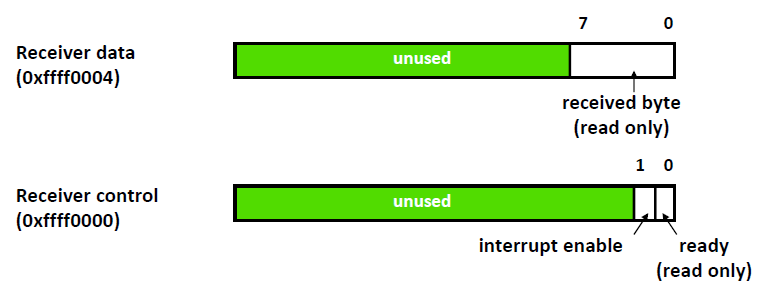
\includegraphics[width=0.9\textwidth,keepaspectratio]{SPIM1}
	\caption{Controllo del terminale in SPIM (INPUT)}
\end{figure}

Le due parole di memoria 0xffff0000 ed 0xffff0004 sono riservate al SO.
La prima è il Receiver control, ovvero viene utilizzata per contenere il bit che segnala la presenza di un nuovo dato in ingresso (ready) e quello per stabilire se l'interrupt è abilitato (vedremo in seguito cosa significa).
La seconda è il Receiver data che conterrà gli effettivi dati forniti in input.

Ora che abbiamo chiarito l'utilizzo di queste due parole in memoria possiamo osservare anche degli esempi di implementazione in MIPS di polling.

Esempio 1: Input, lettura dalla tastiera in \$v0
\begin{minted}{asm}
	lui $t0, 0xffff #0xffff0000
Waitloop:
	lw $t1, 0($t0) #control
	andi $t1,$t1,0x0001
	beq $t1,$zero, Waitloop
	lw $v0, 4($t0) #data
\end{minted}
Analizziamo ora il significato del codice:
l'operazione load upper immediate carica nei bit più significativi del registro t0 ffff, così che esso contenga l'indirizzo del Receiver control.
La lw carica in t1 il Receiver control.
Se è presente il bit ready significa che il dato è pronto e quindi viene caricato in memoria (in \register{\$v0} il carattere effettivamente pigiato, che si trova in 0xffff0004.
Nel caso il bit ready non sia presente il beq farà ripetere il waitloop.

Esempio 2: Output, stampa del dato da \$a0
\begin{minted}{asm}
	lui $t0, 0xffff #0xffff0000
Waitloop:
	lw $t1, 8($t0) #control
	andi $t1,$t1,0x0001
	beq $t1,$zero, Waitloop
	sw $a0, 12($t0) #data
\end{minted}
Nel secondo esempio cambiano solamente le aree di memoria in cui si compie la verifica dato che l'area dedicata alla lettura da tastiera è diversa da quella dedicata alla scrittura su video.
Nonostante ciò il procedimento è simmetrico a quello del primo waitloop osservato.

Osserviamo ora l'aspetto del costo in termini di risorse del meccanismo del polling con i seguenti esempi:
Consideriamo un processore a 500Mhz e supponiamo che occorrano 400 cicli di clock per un’operazione di polling. Qual è il costo percentuale di questo meccanismo?

\paragraph{Esempio 1: Mouse} Per non perdere movimenti da parte dell’utente occorre acquisire il dato 30 volte al secondo.

Per stimare l'impatto del polling sul processore si deve calcolare il numero di clock al secondo spesi per il polling stesso, ovvero \(30*400 = 12000\) clocks/sec.
Ora che abbiamo il numero di clock spesi per il polling ci basta calcolare a che percentuale di utilizzo del processore corrispondono, ricordando che 500Mhz significa \(500*10^{6}\) clocks/sec.
Quindi complessivamente l'impatto del polling in percentuale è \[12*10^{3}/500*10^{6}=0.002\%\]

È chiaro quindi che in questo caso l'impatto del polling è trascurabile, si noti tuttavia che questo overhead viene pagato sempre, sia che avvenga il trasferimento, sia che non avvenga.

\paragraph{Esempio 2: Hard disk} I dati vengono trasferiti in blocchi di 16 byte ad una velocità di 8MB/s senza la possibilità di perdite.

Il numero di volte al secondo che occorre fare cicli di attesa per non perdere dati è \[\frac{8\textrm{MB/s}}{16\textrm{B}} = 500*10^{3} \textrm{polls/sec}\]
Questo implica che il numero di cicli di clock al secondo dedicati al polling siano \[ 500*10^{3}*400 = 200*10^{6} \textrm{clocks/sec}\]
In percentuale quindi il peso di questo meccanismo è di \(200*10^{6}/500*10^{6}=40\%\) il che è inaccettabile, anche perché come nel primo esempio questo prezzo in risorse viene pagato sempre.

\subsection{Considerazioni finali sul polling}
L’attesa attiva è un meccanismo che fa perdere tempo al processore dedicando cicli macchina a letture inutili, di conseguenza il polling può essere usato quando le operazioni di I/O avvengono con velocità di trasferimento predeterminata (es. applicazioni di controllo) e comunque il processore ha poco altro da fare.

Sicuramente se i dati vengono trasferiti con elevati \emph{bitrate}\footnote{Indica la quantità di dati che possono essere trasferiti, su un canale di comunicazione in un dato intervallo di tempo.} il ciclo di attesa attiva dura poco, in altri casi lo spreco derivante dal polling è inaccettabile e per questo motivo è stato inventato il sistema di I/O a interruzione di programma.

Osserviamo ora uno schema esemplificativo tratto dal simulatore SPIM per l'assembly MIPS.
\begin{figure}[!h]
	\centering
	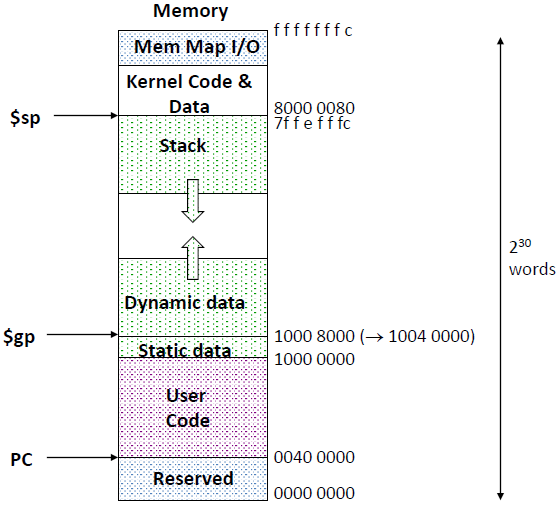
\includegraphics[width=0.8\textwidth,keepaspectratio]{SPIM}
	\caption{Organizzazione memoria SPIM (MIPS)}
\end{figure}

La parte più in alto in questa rappresentazione della memoria è quella che contiene il kernel code e le parole riservate.

Il kernel code è la traduzione in linguaggio macchina del SO (che ricordiamo essere un programma esso stesso); all'interno di questa sezione si trovano inoltre le parole di memoria riservare all I/O; è quindi ora chiaro cosa si intendeva quando si è detto che il processore vede solo virtualmente le periferiche, che fisicamente dal suo punto di vista altro non sono che dati.

\section{Input ad interruzione di programma}
Conosciuto anche con il nome di interrupt driven I/O funziona tramite il sollevamento di interruzioni.

Un’interruzione I/O è un segnale usato per indicare al processore che la periferica è pronta ad eseguire il trasferimento richiesto.
Occorre tuttavia un modo per segnalare al processore quale periferica richiede l’interruzione e per gestire il fatto che le interruzioni I/O sono sempre asincrone rispetto all’esecuzione delle istruzioni.

Non esistono particolari istruzioni assembly per eseguire le interruzioni, queste possono presentarsi mentre una qualsiasi istruzione viene eseguita, ma si deve comunque dare modo di terminare l’esecuzione dell’istruzione corrente prima di passare alla gestione dell'interruzione.
In tal senso il programmatore può decidere di posticipare l’esecuzione dell’interruzione a un momento più conveniente programmando sezioni non interrompibili nel codice del kernel, inoltre può classificare le interruzioni secondo grado di priorità.

Il maggiore vantaggio che deriva dall'utilizzo di questa strategia è che non occorre interrompere l’esecuzione del programma se non quando il dato può essere effettivamente riferito in memoria.

Guardando invece il lato negativo occorre un hardware speciale per permettere ai dispositivi di I/O di generare un’interruzione, rilevare l’interruzione, salvare lo stato del processore per eseguire una particolare routine di servizio (Interrupt Service Routine, ISR) e poi riprendere dal punto dove si era interrotto.

\begin{figure}[!h]
	\centering
	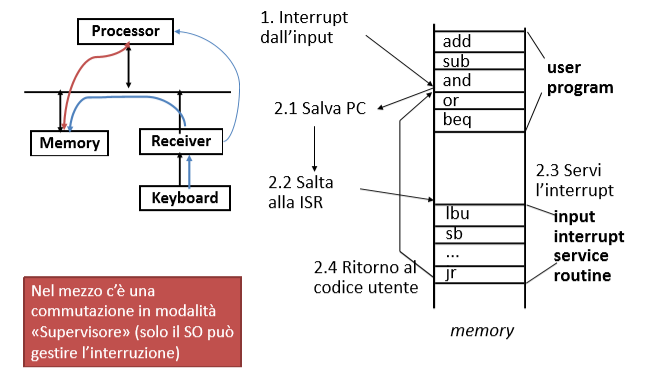
\includegraphics[width=0.9\textwidth,keepaspectratio]{input-a-interruzione}
	\caption{Meccanismo di input ad interruzione}
\end{figure}

È ora presentato un'esempio di implementazione di gestione dell'I/O tramite interrupt in SPIM.
\begin{figure}[!h]
	\centering
	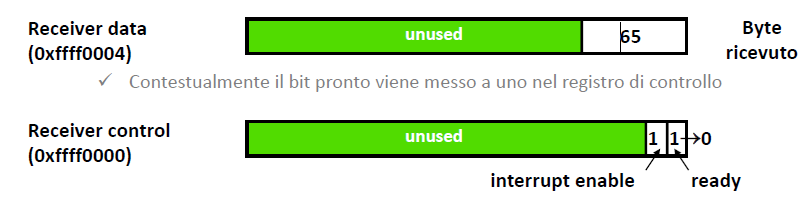
\includegraphics[width=0.9\textwidth,keepaspectratio]{SPIM2}
	\caption{Esempio controllo terminale SPIM}
\end{figure}

In questo esempio si nota come vi sia ancora, come nel polling, una parola dedicata alla segnalazione della presenza di dati da scrivere, il Receiver control (0xffff0000); la parola succcessiva viene utilizzata per memorizzare effettivamente il dato disponibile, il Receiver data (0xffff0004).

La periferica indica con un’interruzione, che viene lanciata da una circuiteria di controllo del bit ready, che ha un nuovo carattere dalla tastiera nell’opportuno registro di ricezione.

Il processo utente viene interrotto trasferendo il controllo a una ISR che copia il dato in memoria utente. Contemporaneamente con la lettura il bit ready viene resettato.

Nel dettaglio il bit interrupt enable serve per indicare se è abilitato il meccanismo di interrupt.

\subsection{Considerazioni finali sull'interrupt driven I/O}
Nonostante la complessità di questo meccanismo è facile osservare che in caso di trasferimenti di grandi moli di dati esso risulti  molto più efficiente del polling, dimostriamolo riprendendo l'esempio dell'hard disk fatto in precedeza:

\paragraph{Esempio 2: Hard disk} Supponiamo che un interrupt costi 500 cicli di clock, poiché è plausibile che costi di più del polling.
Se le interruzioni venissero generate alla frequenza di polling avremmo che \[\frac{\textrm{Disk Interrupts}}{\textrm{sec}}=\frac{8 \textrm{MB/s}}{16\textrm{B}}=500*10^{3}\frac{\textrm{interrupts}}{\textrm{sec}}\] e quindi \[\frac{\textrm{Disk Polling Clocks}}{\textrm{sec}}=500*10^3{3}*500=250*10^{6} \frac{\textrm{clocks}}{\textrm{sec}}\] Di conseguenza la percentuale di utilizzo del processore sarebbe \(250*10^{6}/500*10^{6}= 50\%\). Sembrerebbe che non ci sia guadagno, anzi.

Tuttavia se l’hard disk è attivo solo per il 5\% del tempo, gli interrupt generati saranno il 5\% e la spesa di processore sarà: \(5\% * 50\%=2.5\%\).

Tutto questo proprio grazie al fatto che con il meccanismo di interrupt l’overhead si paga solo quando vengono effettivamente generate richieste.

\section{Eccezioni}
Le interrupts che abbiamo appena visto vanno inserite in una classe più grande di eventi detti eccezioni.

Un eccezione consiste nel trasferimento del controllo del programma per l'avveramento di una condizione appunto eccezionale\footnote{Da intendere qui come "fuori dalla norma".}.
Per la gestione di questi eventi il sistema effettua delle azioni specifiche, come registrare il punto di interruzione e salvare lo stato, ed in seguito, a eccezione finita, riprendere dal punto immediatamente successivo al punto di interruzione.

\begin{figure}[!h]
	\centering
	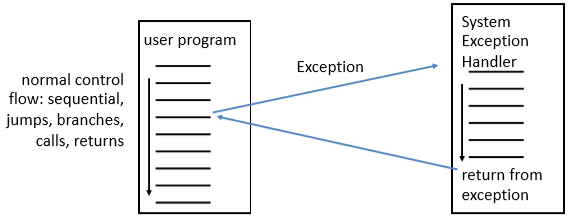
\includegraphics[width=0.9\textwidth,keepaspectratio]{schema-eccezioni}
	\caption{Schema processo delle eccezioni}
\end{figure}

Esistono due tipi di eccezioni:
\paragraph{Interrupts} Sono causate da eventi esterni (I/O) e quindi sono asincrone; possono essere gestite nello spazio tra due istruzioni semplicemente sospendendo il programma e riprendendo, dopo la gestione, dal punto in cui era stato interrotto.
\paragraph{Traps} Sono causate da eventi \emph{interni} al programma come condizioni eccezionali (es. arithmetic overflow), errori (es. hardware malfunction) o fault (es. page fault).
Esse sono sincrone all’esecuzione del programma.
Vengono gestite da un \emph{traphandler}, da notare che spesso è possibile riprovare ad eseguire l’istruzione che ha causato l’eccezione o abortire il programma.

\subsection{Supporto del MIPS per la gestione di eccezioni}
La componenete che registra le informazioni necessarie alla gestione delle eccezioni in MIPS è il coprocessore 0, che utilizza dei registri a lui dedicati.

Quando si presenta un'eccezione in MIPS il registro EPC (registro 14) punta all’indirizzo successivo all’istruzione in esecuzione quando l’eccezione è avvenuta, mentre il registro di stato (registro 12) fa da maschera di abilitazione trap/interrupt.

\begin{figure}[!h]
	\centering
	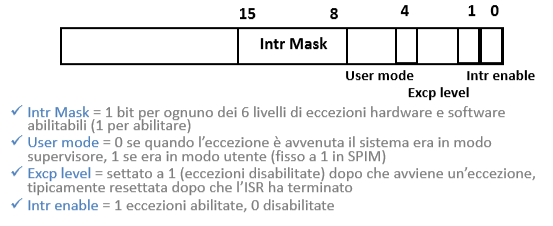
\includegraphics[width=0.9\textwidth,keepaspectratio]{registro-maschera}
	\caption{Registro maschera}
\end{figure}

In seguito una breve spiegazione dei campi di questo registro.
\begin{itemize}
	\item IntrMask:  1 bit per ognuno dei 6 livelli di eccezioni hardware e 2 livelli software abilitabili.
	\item User mode: 0 se quando l’eccezione è avvenuta il sistema era in modo supervisore, 1 se era in modo utente.
	\item Excp level: settato a 1 (eccezioni disabilitate) mentre si stà gestendo un’eccezione, tipicamente resettata dopo che l’ISR ha terminato.
	\item Intr enable: 1 se si sta utilizzando il meccanismo delle interrupt, 0 altrimenti.
\end{itemize}

Il registro BadVAddr (registro 8) contiene l'indirizzo di memoria che ha causato un errore di memoria.
Infine il registro cause (registro 13) contiene il tipo dell’eccezione ed i bit pendenti.

\begin{figure}[!h]
	\centering
	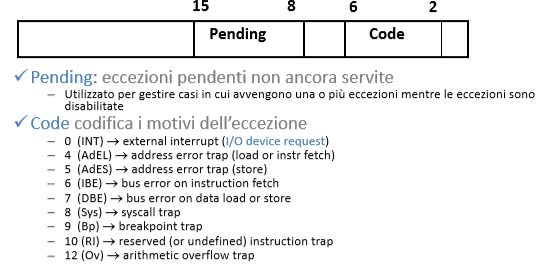
\includegraphics[width=0.9\textwidth,keepaspectratio]{registro-cause}
	\caption{Registro cause}
\end{figure}

In particolare sono importanti i campi:
\begin{itemize}
	\item \textbf{code}, che codifica i motivi dell'eccezione;
	\item \textbf{pending}, utilizzato per gestire casi in cui avvengono una o più eccezioni mentre venivano risolte altre eccezzioni.
\end{itemize}

\subsection{Modifiche al processore per gestire le eccezioni}
Per implementare il complesso meccanismo di gestione delle eccezioni il processore deve essere munito di queste nuove componenti:
\begin{itemize}
	\item segnali di controllo per scrivere EPC (EPCWrite), Cause (CauseWrite) e Status;
	\item hardware per registrare il tipo di interruzione in Cause;
	\item modifiche alla macchina a stati in modo che:
	\begin{itemize}
		\item l’indirizzo del gestore dell’interruzione, 0x80000180  possa essere caricato in PC (altro ramo nel multiplexer);
		\item Sia salvato l’indirizzo della prossima istruzione da eseguire a ISR terminato in EPC.
	\end{itemize}
\end{itemize}

Ed ecco infine un'immagine del processore con dattapath modificato per supportare la gestione delle eccezioni.

\begin{figure}[!h]
	\centering
	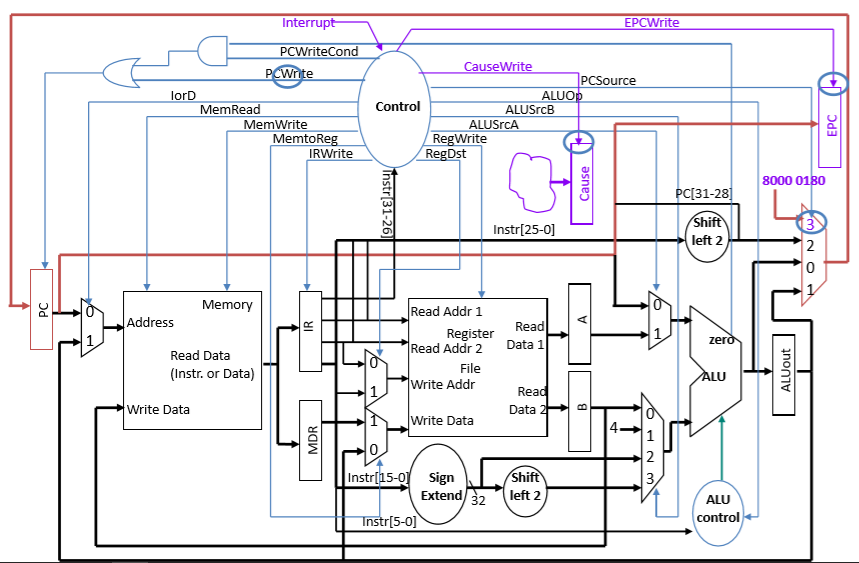
\includegraphics[width=0.9\textwidth,keepaspectratio]{final-datapath}
\end{figure}

\end{document}
